% Facultad de Ingenier�a, Universidad de Buenos Aires
% 75.10 T�cnicas de dise�o

\documentclass[12pt]{article}
\usepackage[a4paper]{geometry}
\usepackage[spanish]{babel}
\usepackage[latin1]{inputenc}
\usepackage{graphicx}
\graphicspath{{../}}

\usepackage{listingsutf8}

\title{75.10 T�cnicas de Dise�o, TP Grupal}
\author{Awad, Lucas \and Choque, Javier \and L�pez, Federico \and Rodriguez, Leandro}
\date{ \today }

\begin{document}

\maketitle

\section{Hip�tesis y supuestos}

Para la realizaci�n del trabajo pr�ctico se tomaron las siguientes hip�tesis:
\begin{itemize}
%	\item Cada producto puede aplicar s�lo para una oferta. 
	\item Cada oferta genera un descuento monetario sobre el valor final de la venta.
	\item Existe una �nica sucursal, con una �nica caja.
	\item No se persiste ninguno de los datos generados durante la ejecuci�n del programa.
\end{itemize}

\section{Ofertas}

\subsection{Tipos}
Las ofertas fueron clasificadas en 3 categor�as:
\begin{itemize}
	\item Por unidad, ya sea marca, categor�a o producto.
	\item Por volumen.
	\item Por medio de pago.
\end{itemize}

\subsection{Generaci�n de ofertas}
La casa central del hypermercado, que es la generadora de ofertas, las env�a a cada sucursal para su aplicaci�n. Dado que la modelizaci�n de dicho comportamiento no es parte del alcance del presente trabajo pr�ctico, las ofertas est�n representadas en archivos de texto. Para el agregado de nuevas ofertas se deben modificar dichos archivos, que son cargados peri�dicamente durante la ejecuci�n del programa.

Por cada tipo de oferta existe un archivo distinto.

\subsection{Aplicaci�n de ofertas}
Las condiciones que se deben cumplir para poder aplicar las ofertas en cada caso son diferentes. Debido a la necesidad de variar el comportamiento se implemento el patr�n $Strategy$.

En las ofertas, el comportamiento que varia es la decisi�n sobre si la oferta puede o no aplicarse a un producto. Entonces, cada oferta tiene una colecci�n de criterios de selecci�n de productos (por marca, por categoria de producto, etc). Para saber si una oferta aplica, se debe aplicar el metodo $encajaEnOferta$ de cada uno de los criterios sobre el producto. �ste devuelve un valor l�gico que se debe comparar con todos los criterios.

\begin{figure}[htbp!]
\begin{center}
	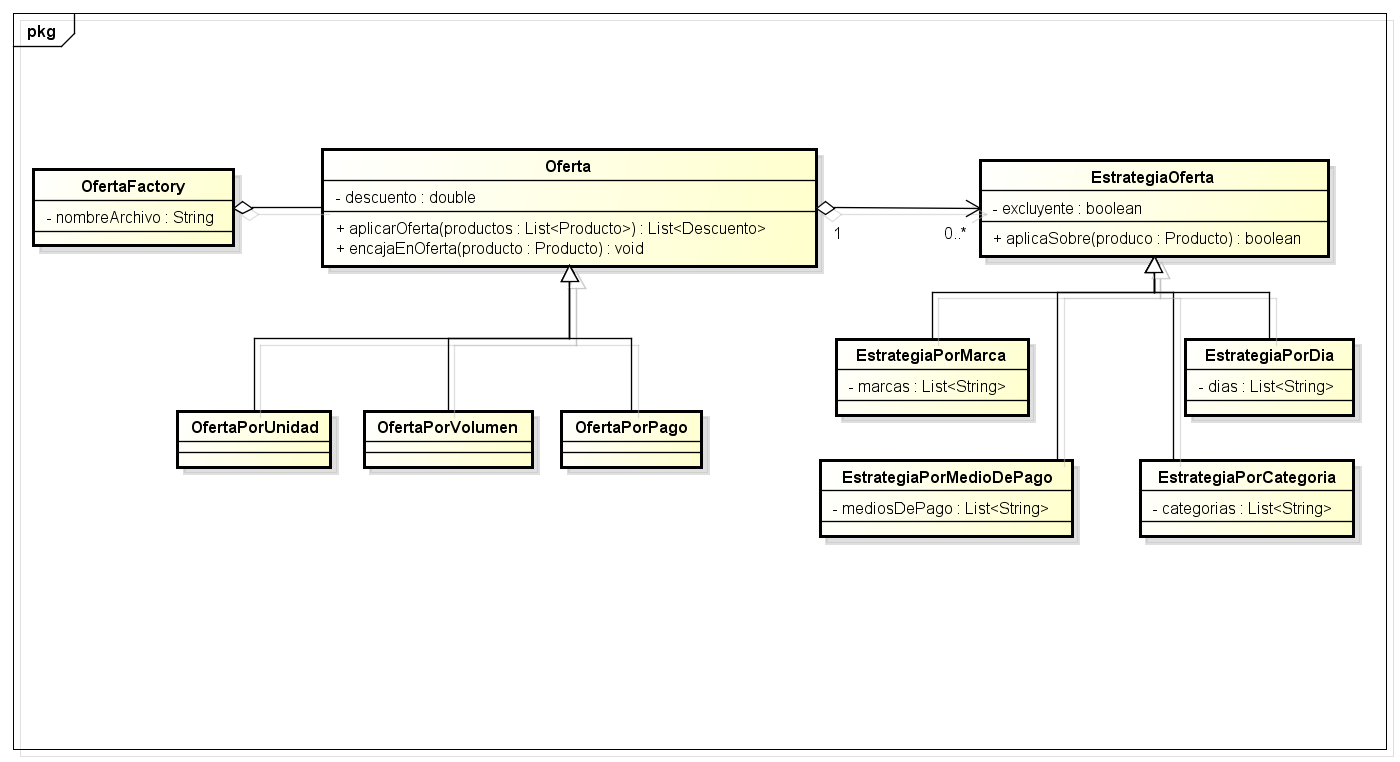
\includegraphics[width=\textwidth]{diagramaOfertas.png}
	\caption{Diagrama del patr�n $Strategy$ aplicado a las ofertas.}
\end{center}
\end{figure}


\section{Extensi�n del sistema}
Tras el objetivo de cumplir con el principio de una implementaci�n clausurada ante cambios y abierta a extensiones, se desarroll� una jer�rquia de ofertas en conjunto con la aplicaci�n de patr�n $Strategy$. 
Se busc� que la aparici�n de nuevos tipos de ofertas pueda ser tratada agregando las clases correspondientes, y sin modificar las preexistentes.  

Entonces, para crear una nueva oferta, se debe crear un objeto OfertaIndividual, y agregarle los criterios que lo definen. Los criterios son, por defecto, inclusivos, es decir, representan una condici�n que debe cumplirse. Pero pueden definirse criterios  \textit{excluyentes}, o sea, los productos que coincidan, no entran en la oferta.

A continuaci�n damos unos ejemplos:

\begin{itemize}
	\item Supongamos que queremos una nueva oferta del 10\% en jugos \textit{Rinde dos}. Al objeto OfertaIndividual, le agregamos un criterio por marca, para la marca \textit{Rinde dos}, y le establecemos un valor del 10\%.
	\item Ahora queremos una oferta para todas las bebidas, del 15\%. Creamos una oferta individual, y le agregamos un criterio por categoria, de la categoria \textit{Bebidas}.
	\item Para un descuento del 12\% en bebidas, \textit{excepto} la marca Chandon, debemos crear una oferta individual, agregarle el criterio de categoria ''bebidas'', y agregarle un criterio de marca ''Chandon'', excepto que a �ste criterio debemos setearle la condici�n de \textit{excluyente}.
	\item Queremos una oferta de 2x1 en bebidas. Simplemente agregamos un criterio de selecci�n de productos por categor�a, a una oferta por volumen.
\end{itemize}

\end{document}
